\subsubsection{Test Case 1}
A comparison was conducted for a hollow cylinder undergoing uniform flow with
acoustic liners along the outer duct perimeter. The azimuthal mode number, reduced 
frequency, mach number and duct liner admittance is reported below,
\begin{align*}
    m &= 2 \\
    k &= \frac{\omega r_T}{A_T} = -1 \\
    M_x &= 0.5 \\
    \eta_T &= 0.72 + 0.42i\\
    \sigma &= 1
\end{align*} 

% \begin{figure}[h!]
%     \centering
%     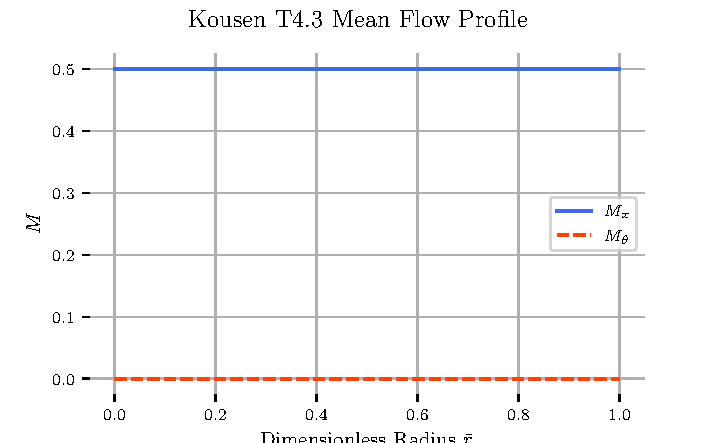
\includegraphics{/home/jeff-severino/SWIRL/CodeRun/04-plotReport/tex-outputs/KousenT1_mean_flow_profile.pdf}
%     \caption{Mean mach number profile for the uniform flow in a lined cylinder}
%     \label{fig:1}
% \end{figure}


\begin{figure}[h!]
    \centering
    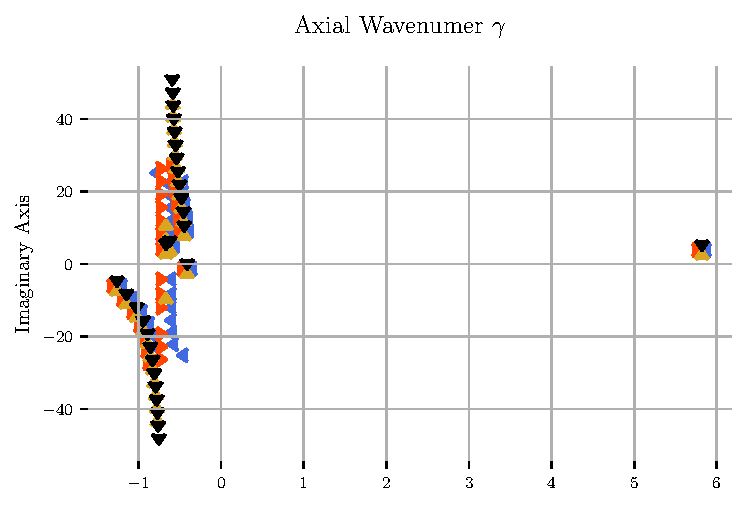
\includegraphics[width=\textwidth]{/home/jeff-severino/SWIRL/CodeRun/04-plotReport/tex-outputs/KousenT1_gam_nonconv_scatter_2ndOrderApprox.pdf}
\end{figure}



% \begin{figure}[h!]
%     \centering
%     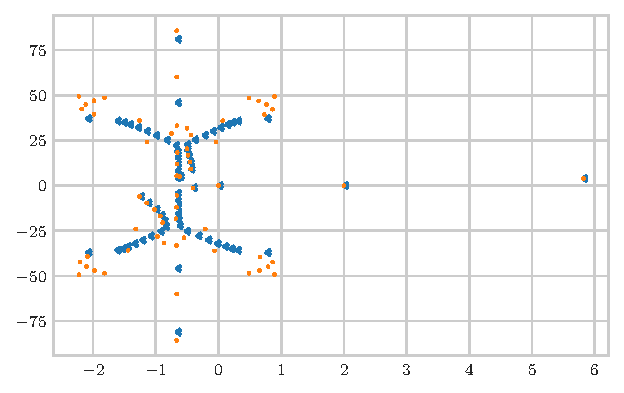
\includegraphics[width=\textwidth]{/home/jeff-severino/SWIRL/CodeRun/04-plotReport/tex-outputs/gam.nonconv.scatter_2nd_ord_32pts.pdf}
% \end{figure}

% \begin{figure}[h!]
%     \centering
%     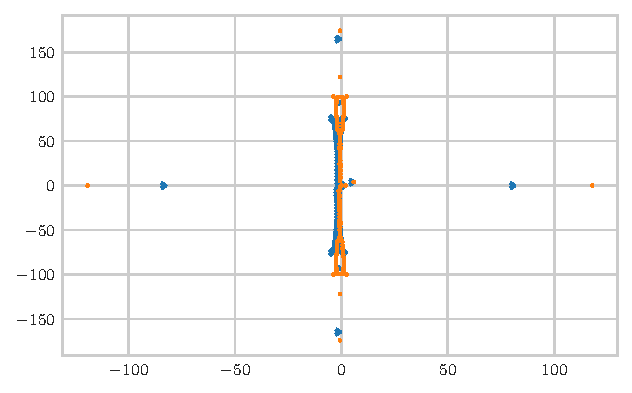
\includegraphics[width=\textwidth]{/home/jeff-severino/SWIRL/CodeRun/04-plotReport/tex-outputs/gam.nonconv.scatter_2nd_ord_64pts.pdf}
% \end{figure}


% \begin{figure}[h!]
%     \centering
%     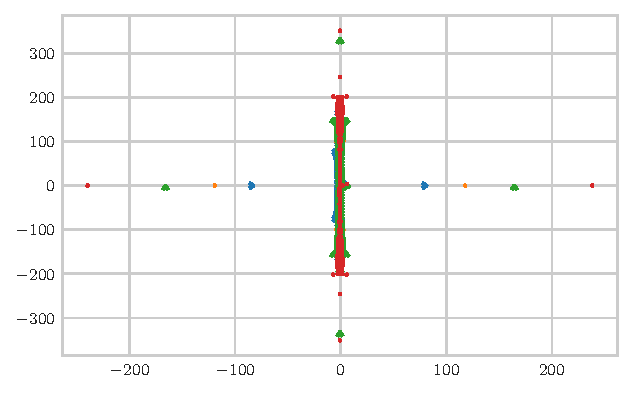
\includegraphics[width=\textwidth]{/home/jeff-severino/SWIRL/CodeRun/04-plotReport/tex-outputs/gam.nonconv.scatter_2nd_ord_128pts.pdf}
% \end{figure}

\begin{figure}[h!]
    \centering
    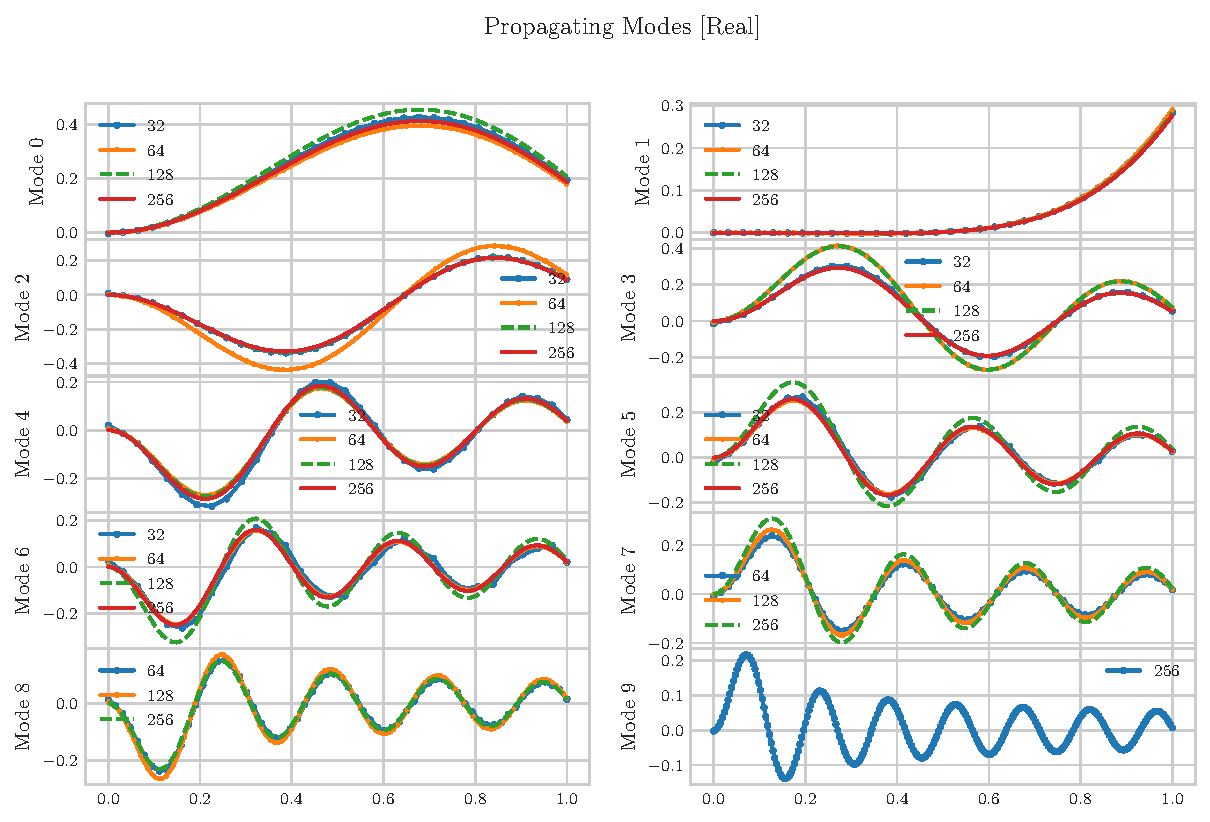
\includegraphics[width=\textwidth]{/home/jeff-severino/SWIRL/CodeRun/04-plotReport/tex-outputs/egv_prop_re.pdf}
    \label{fig:prop_re}
\end{figure}

\begin{figure}[h!]
    \centering
    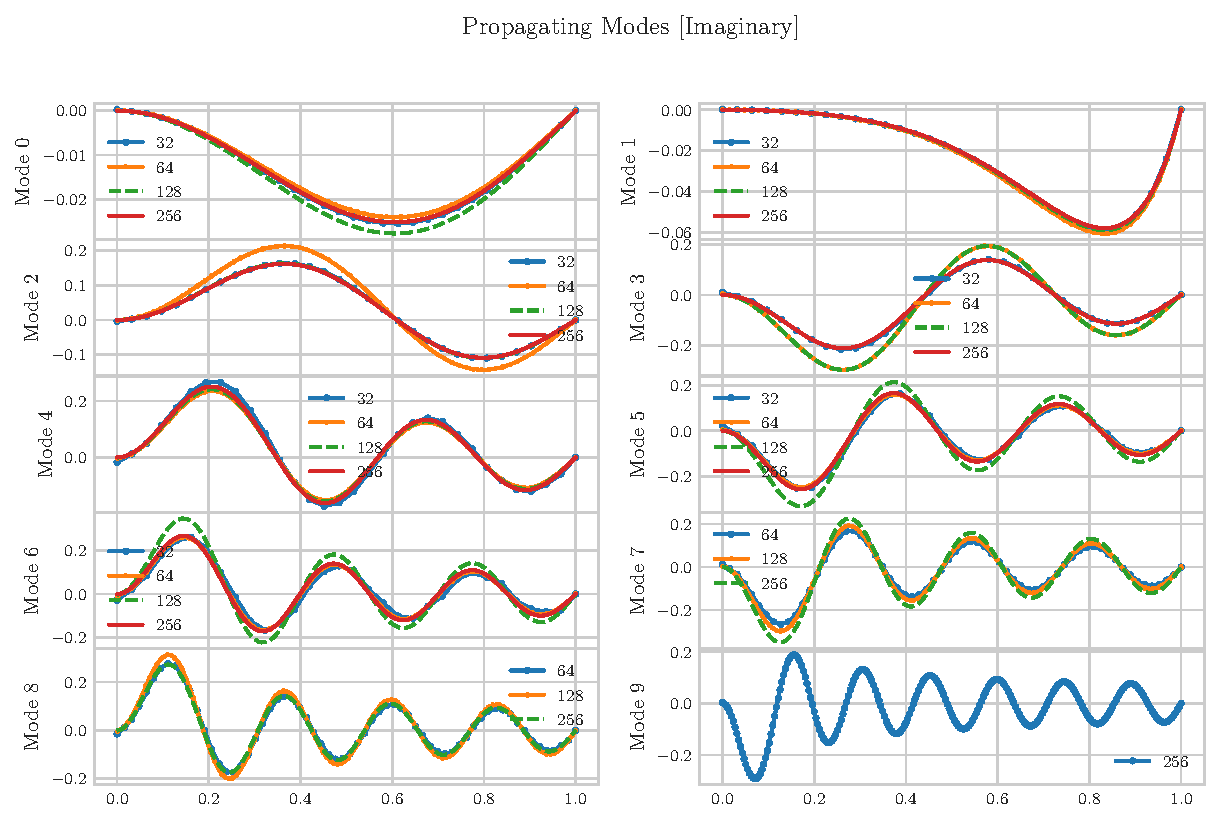
\includegraphics[width=\textwidth]{/home/jeff-severino/SWIRL/CodeRun/04-plotReport/tex-outputs/egv_prop_im.pdf}
    \label{fig:prop_im}
\end{figure}

\begin{figure}[h!]
    \centering
    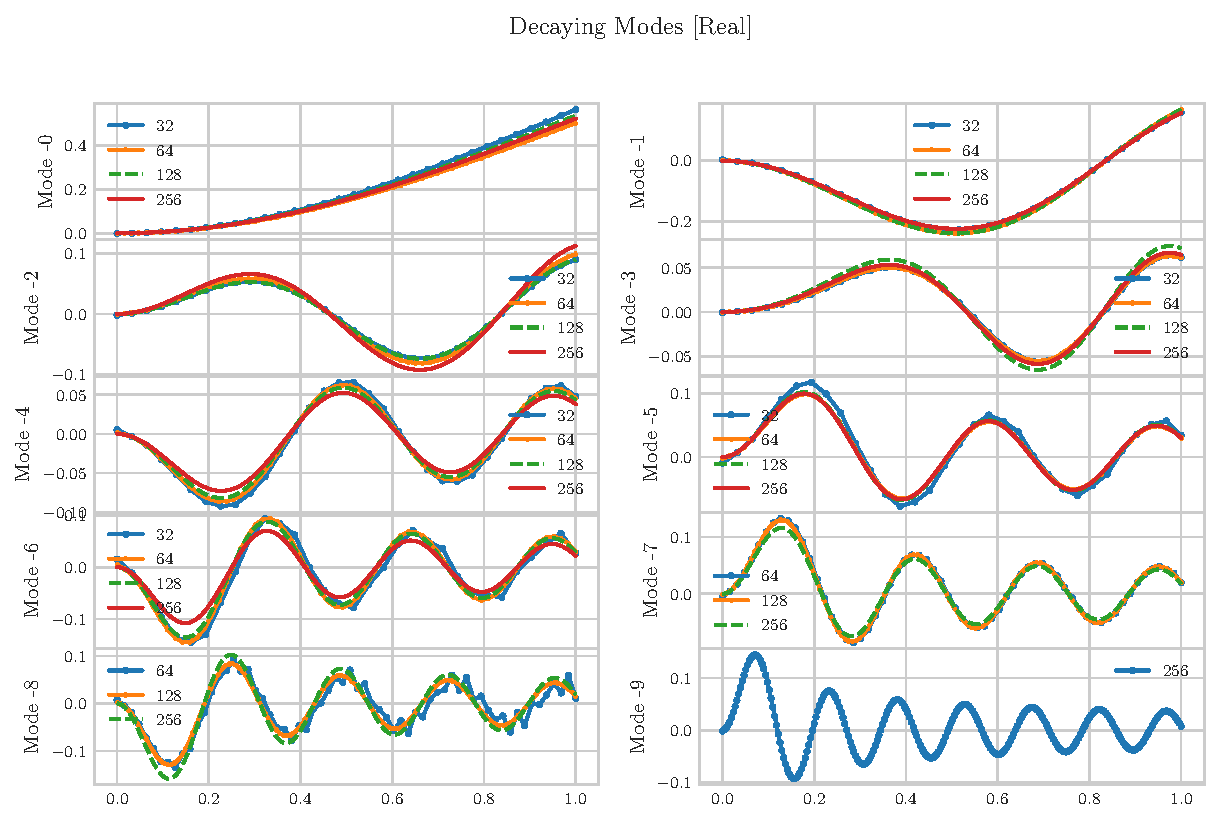
\includegraphics[width=\textwidth]{/home/jeff-severino/SWIRL/CodeRun/04-plotReport/tex-outputs/egv_decay_re.pdf}
    \label{fig:decay_re} 
\end{figure}

\begin{figure}[h!]
    \centering
    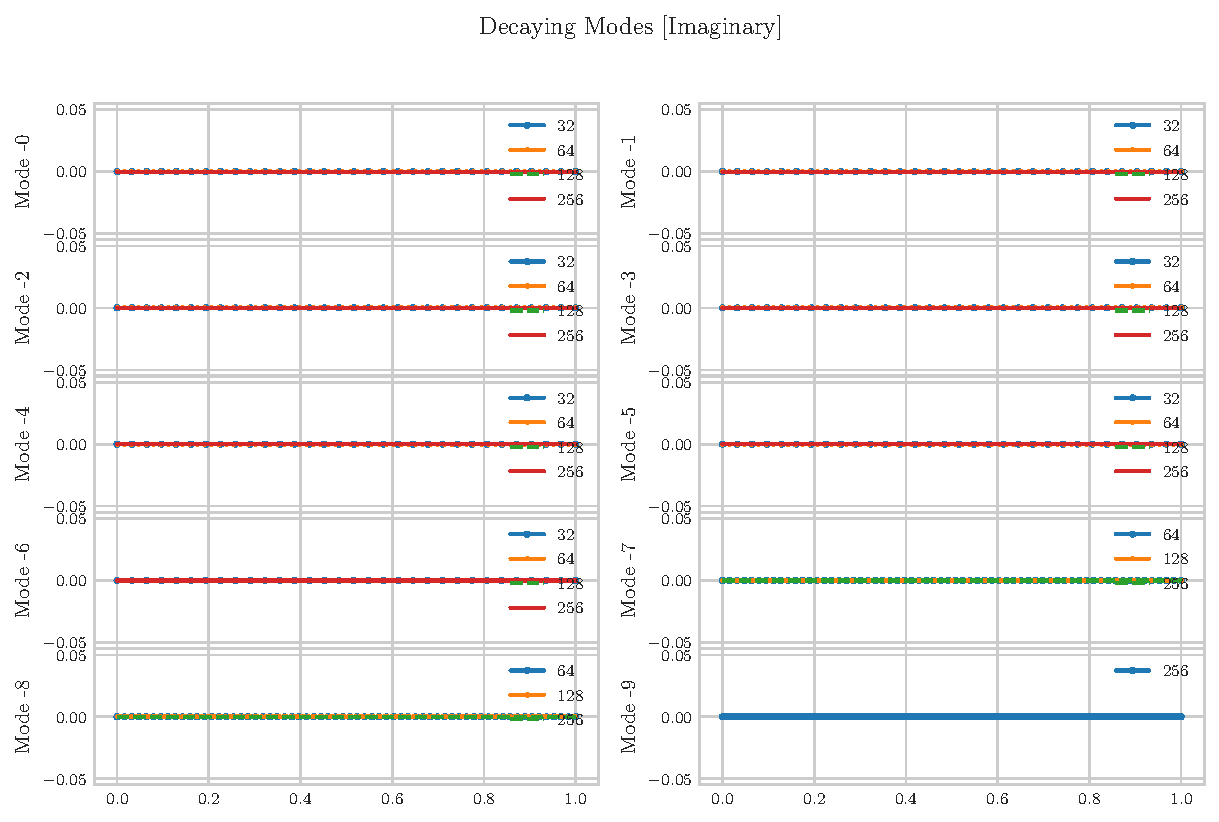
\includegraphics[width=\textwidth]{/home/jeff-severino/SWIRL/CodeRun/04-plotReport/tex-outputs/egv_decay_im.pdf}
    \label{fig:decay_im} 
\end{figure}








The results shown in \ref{Table43} are in moderately good agreement. The 
results were obtained by visually comparing the output for 32 
grid points. Note that the indicies for the SWIRL deliverable are different that 
the ones obtained for the most recent version of the code. While the 
convective axial wavenumbers show agreement to machine precision, this is not 
particularly insightful given that there are an infinite number of possible solutions 
that could satisfy the eigenvalue problem. The results that are of concern 
are propagating modes that are not convecting with the mean flow.  The scatter plot
of the axial wavenumbers show some sporadic behaviour around the imaginary axis.
The results from the MMS along with this plot indicate that more grid points are going 
to be needed if a finite difference technique is to be used.

The first 10 propagating and decaying modes are plotted in \ref{fig:prop_re}-\ref{fig:decay_im}.



% It should be 
% noted that a spectral differencing method were using for Kousen's report and for
% srcF2008. 
%Using a higher order scheme would also improve accuracy.


\begin{table}
 \centering
 \begin{adjustbox}{width=1\textwidth}
     \small
\begin{tabular}{c | r | r | r }
 \hline
 $\gamma^{\pm}_n$ & Kousen Ref. [15] & Kousen report &   current  \\
 \hline
 $\gamma_0^{+}$ & $ 0.620 - 5.014  i $ & $ 0.6195 - 5.0139 i$ & 0.620755853112 - 5.00592416941i  \\
 $\gamma_1^{+}$ & $-5.820 - 3.897  i $ & $-5.8195 - 3.8968 i$ &-0.581267772517 - 3.90050864568i \\
 $\gamma_2^{+}$ & $ 0.445 - 9.187  i $ & $ 0.4453 - 9.1868 i$ &0.451569491142 -  9.12191317214i\\
 $\gamma_3^{+}$ & $ 0.453 - 13.062 i $ & $ 0.4539 - 13.062 i$ &0.464247902898 - 12.8487472519i \\ 
 $\gamma_4^{+}$ & $ 0.480 - 16.822 i $ & $ 0.4795 - 16.822 i$ &0.492340380223 - 16.3292825150i \\
 % $\gamma_5^{+}$ & $ 0.503 - 20.531 i $ & $ 0.5029 - 20.531 i$ &0.514522630594 -19.5817182568i \\
 % $\gamma_6^{+}$ & $ 0.522 - 24.213 i $ & $ 0.5220 - 24.213 i$ &0.516658239854 -22.5715880605i \\
 % $\gamma_7^{+}$ & $ 0.538 - 27.880 i $ & $ 0.5376 - 27.880 i$ & -  \\
 % $\gamma_8^{+}$ & $ 0.550 - 31.537 i $ & $ 0.5502 - 31.537 i$ & -  \\
 % $\gamma_9^{+}$ & $ 0.589 - 49.75  i $ & $ 0.5891 - 49.754 i$ &-  \\ \hline
 $\gamma_0^{-}$ & $ 0.410 + 1.290  i $ & $ 0.4101 + 1.2904 i$ &0.409973310292  + 1.29020083859i\\
 $\gamma_1^{-}$ & $ 1.259 + 6.085  i $ & $ 1.2595 + 6.0852 i$ &1.25530612217  + 6.07214375548i \\
 $\gamma_2^{-}$ & $ 1.146 + 9.668  i $ & $ 1.1457 + 9.6679 i$ &1.13696444935  + 9.59622801724i \\
 $\gamma_3^{-}$ & $ 1.022 + 13.315 i $ & $ 1.0218 + 13.315 i$  &1.00950576515 + 13.0957277529i \\
 $\gamma_4^{-}$ & $ 0.943 + 16.977 i $ & $ 0.9425 + 16.977 i$  &0.928059983039 +  16.4791343118i\\ \hline
 % $\gamma_5^{-}$ & $ 0.891 + 20.635 i $ & $ 0.8908 + 20.635 i$    &0.856678172769 +  22.6544943903i \\
 % $\gamma_6^{-}$ & $ 0.855 + 24.288 i $ & $ 0.8549 + 24.288 i$    &0.941762848775 +  25.3460188358i \\
 % $\gamma_7^{-}$ & $ 0.829 + 27.937 i $ & $ 0.8288 + 27.937 i$    &-  \\
 % $\gamma_8^{-}$ & $ 0.809 + 31.581 i $ & $ 0.8089 + 31.581 i$    &-  \\
 % $\gamma_9^{-}$ & $ 0.755 + 49.77  i $ & $ 0.7547 + 49.772 i$    &-  \\ \hline
 \end{tabular}
\end{adjustbox}
\caption{Cylindical duct with Uniform flow, $M_x = 0.5$ and Acoustic Liner $\eta_{T} = 0.72 + 0.42i$, $k = -1$, and $m=2$}
 \label{Table43}
\end{table}

